\documentclass[10pt,twocolumn]{article}
\usepackage[margin=0.8in]{geometry}
\usepackage{graphicx,booktabs,amsmath,hyperref,xcolor,microtype}
\usepackage[numbers]{natbib}
% generated by recall/bench/paper_numbers.py from results/ — do not edit
\newcommand{\RecallLoc}{0.25}
\newcommand{\PriorLoc}{0.30}
\newcommand{\RecallLocSub}{0.24}
\newcommand{\BoneLoc}{0.33}
\newcommand{\RecallMinusBone}{-0.09}
\newcommand{\RecallMinusBoneLo}{-0.20}
\newcommand{\RecallMinusBoneHi}{0.01}
\newcommand{\RecallHallSub}{0.10}
\newcommand{\BoneHall}{0.75}
\newcommand{\HallDiff}{0.65}
\newcommand{\HallDiffLo}{0.51}
\newcommand{\HallDiffHi}{0.78}
\newcommand{\ObjHeadVal}{0.17}
\newcommand{\NTrainVideos}{27}
\newcommand{\NValVideos}{10}
\newcommand{\NTestVideos}{21}
\newcommand{\NWhere}{507}
\newcommand{\NTemporal}{243}
\newcommand{\NState}{163}
\newcommand{\NAbsent}{63}
\newcommand{\TriggerAbstract}{}
\newcommand{\StorageAbstract}{}
\newcommand{\CalibAbstract}{}
\newcommand{\HoiHandF}{0.92}
\newcommand{\HoiContactF}{0.87}
\newcommand{\HoiContactFQ}{0.82}
\newcommand{\EmbMBfp}{144.1}
\newcommand{\EmbMBq}{\textcolor{red}{[pending]}}
\newcommand{\EmbCosQ}{\textcolor{red}{[pending]}}
\newcommand{\EmbCosFour}{0.27}
\newcommand{\FaceAll}{0.06}
\newcommand{\FaceLarge}{0.95}
\newcommand{\ScreenAll}{0.15}

\title{Recall: On-Device Episodic Visual Memory with a Learned Trigger,\\ Compact Event Memory and Calibrated Answers}
\author{Eshaan Kapooswalla}
\date{Draft --- generated from \texttt{results/} (every number in this document is a macro written by \texttt{recall/bench/paper\_numbers.py})}
\begin{document}
\maketitle

\begin{abstract}
We ask whether a phone- or glasses-class device can keep a full-day, queryable episodic memory of what its camera saw ---
``where did I leave my keys?'', ``did I turn off the stove?'' --- within a battery budget of about 5\,\%/hour and under
1\,GB/week of storage, while answering more accurately than a large vision--language model (VLM) given sampled video and
than frame sampling with CLIP retrieval. Recall combines (i) a tiny always-on \emph{learned trigger} that decides when to
run heavier perception, (ii) a \emph{compact event memory} of object--place--time records instead of video, and (iii)
\emph{calibrated, evidence-grounded answers} that abstain when memory is insufficient. On a participant-disjoint
EPIC-KITCHENS-100 evaluation with narration-derived ground truth, the answer is mixed. Recall's object-location
accuracy (\RecallLoc{} on the full test set) does not exceed a trivial location prior (\PriorLoc) or a locally run
8B-parameter VLM on a matched subsample (\BoneLoc{} vs.\ \RecallLocSub), but Recall names a place for a never-seen object
only \RecallHallSub{} of the time versus \BoneHall{} for the VLM. \TriggerAbstract{} \StorageAbstract{} \CalibAbstract{}
Energy figures are \emph{estimated} from an explicit model because no phone was available. We release code, configs and
derived metrics, and identify object identity from small egocentric crops as the binding constraint.
\end{abstract}

\section{Introduction}
Wearable cameras have long been proposed as memory aids~\citep{hodges2006sensecam}. Large egocentric datasets such as
Ego4D's episodic-memory benchmarks~\citep{grauman2022ego4d} and EPIC-KITCHENS~\citep{damen2022rescaling} made the
``where did I last see X'' question measurable, and modern VLMs can answer it from sampled frames. Yet the natural
system --- stream or store video and ask a large model later --- violates three constraints that matter for a personal
device: privacy (the day's video leaves the device), storage (video grows with hours), and trust (large models answer
confidently even when the object never appeared).

We study the opposite design point: everything on device, most frames never processed by a large model, memory as a
small graph of events, and answers that carry calibrated confidence and the supporting frame. Our contributions are
the system and an honest, reproducible evaluation of its three components: a learned memory trigger
(\S\ref{sec:trigger}), a compact event memory (\S\ref{sec:memory}), and calibrated, grounded answering
(\S\ref{sec:calib}), together with model compression to LiteRT (\S\ref{sec:compress}), a privacy layer
(\S\ref{sec:privacy}) and an energy analysis (\S\ref{sec:energy}). We report negative results where we find them.

\section{Related Work}
\textbf{Egocentric episodic memory.} Ego4D defines episodic-memory tasks --- visual queries, natural-language queries
(NLQ) and moments~\citep{grauman2022ego4d}; NLQ baselines adapt span localisation such as VSLNet~\citep{zhang2020vslnet}.
EPIC-KITCHENS-100~\citep{damen2022rescaling} supplies dense, participant-written narrations that we turn into
object-location, state and temporal queries. Long-video QA benchmarks such as EgoSchema~\citep{mangalam2023egoschema}
target holistic understanding rather than ``last seen'' retrieval.
\textbf{Hand--object interaction} detection at scale~\citep{shan2020understanding} provides the contact signal our events
are built on. \textbf{Vision--language retrieval}: CLIP~\citep{radford2021clip} and its mobile variants
MobileCLIP~\citep{vasu2024mobileclip} underpin our embeddings and the frame-retrieval baseline; open-vocabulary detection
(e.g.\ OWLv2~\citep{minderer2023owlv2}) and tracking (ByteTrack~\citep{zhang2022bytetrack}) are natural extensions.
\textbf{On-device ML}: efficient backbones~\citep{howard2019mobilenetv3}, distillation~\citep{hinton2015distilling} and
integer quantisation~\citep{jacob2018quantization}; continuous mobile vision is energy-bound by image sensing
itself~\citep{likamwa2013energy}, and smartphone power is dominated by a few components~\citep{carroll2010power}.
\textbf{Memory-augmented agents} store and retrieve experiences for LLM agents~\citep{park2023generative,packer2023memgpt};
we store perceptual events with explicit provenance. \textbf{Calibration and selective prediction}: temperature and
isotonic calibration~\citep{guo2017calibration,zadrozny2002isotonic} and risk--coverage analysis~\citep{geifman2017selective}.

\section{System Design}
Frames arrive at 2\,fps. The \textbf{trigger} $\mu$ is a causal CNN over $36{\times}64$ thumbnails, frame differences and,
when present, IMU statistics; when its score exceeds a budget-calibrated threshold it opens a short burst of heavy
processing. \textbf{Heavy perception} runs a hand--object student (MobileNetV3-Small distilled from the Faster R-CNN
detector of~\citep{shan2020understanding}) and MobileCLIP2-S2 embeddings of the held object and of the context around
where it was released. An \textbf{event extractor} with hysteresis turns contact bouts into \texttt{take}, \texttt{put}
and \texttt{touch} events. Before anything is stored, a \textbf{redactor} pixelates faces (BlazeFace~\citep{bazarevsky2019blazeface})
and screen/document-like regions in the event thumbnail. The \textbf{memory} is a SQLite/SQLCipher database with
\texttt{events}, online object and place clusters, and a \texttt{last\_seen} index. \textbf{Answering} parses the question,
scores candidate events by object posterior (blend of a zero-shot text bank and a linear probe), selects one by a
val-tuned rule, computes features (score margin, conflicts, age, location certainty, \ldots), maps them to a calibrated
probability, and renders a templated answer naming only places present in the chosen evidence; an optional small LLM
rephrase is accepted only if it introduces no new place.

\section{Experimental Setup}
\textbf{Data.} Ego4D access was unavailable, so we use EPIC-KITCHENS-100 with participant-disjoint splits of
\NTrainVideos{} / \NValVideos{} / \NTestVideos{} videos (train/val/test). Ground truth comes from narrations: the last
``put X in/on Y'' before the query time gives the object's place and time; ``turn on/off X'' gives appliance state;
the last ``<verb> X'' gives temporal queries; objects never narrated in a video form \emph{absent} queries whose correct
answer is to abstain. The test set holds \NWhere{} where, \NTemporal{} temporal, \NState{} state and \NAbsent{} absent
queries. All thresholds and answer rules are tuned on val; calibrators are fit on val; nothing is tuned on test.
\textbf{Baselines.} B0: always the most frequent train/val place. B1: Qwen3-VL-8B (4-bit, run locally) given 16 frames
sampled up to the query time and a closed place list. B2: one frame every $N$\,s with CLIP retrieval. B3: a simulated
user who tags put-downs with probability $q$. B4: oracle trigger at narrated moments.
\textbf{Statistics.} 95\,\% cluster-bootstrap CIs resampling videos; paired bootstrap for differences.

\section{Results: Where Is X?}
\begin{figure}[t]\centering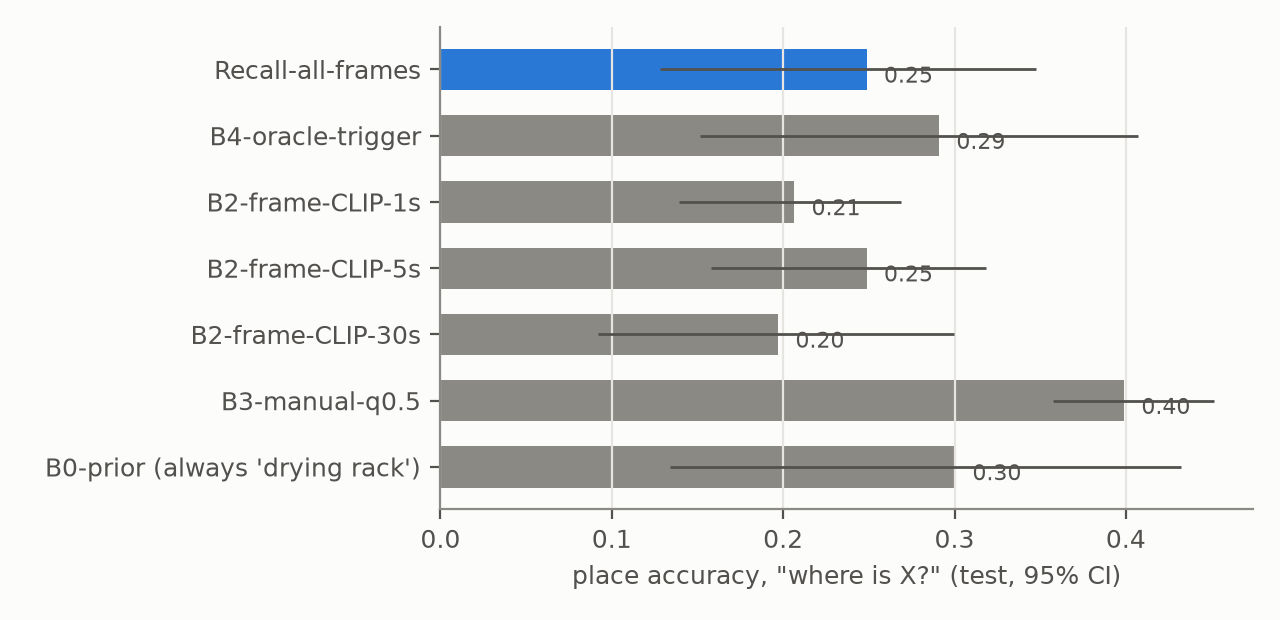
\includegraphics[width=\linewidth]{figs/where_acc.png}
\caption{Place accuracy on the test set (95\,\% CI).}\label{fig:m1}\end{figure}
\begin{figure}[t]\centering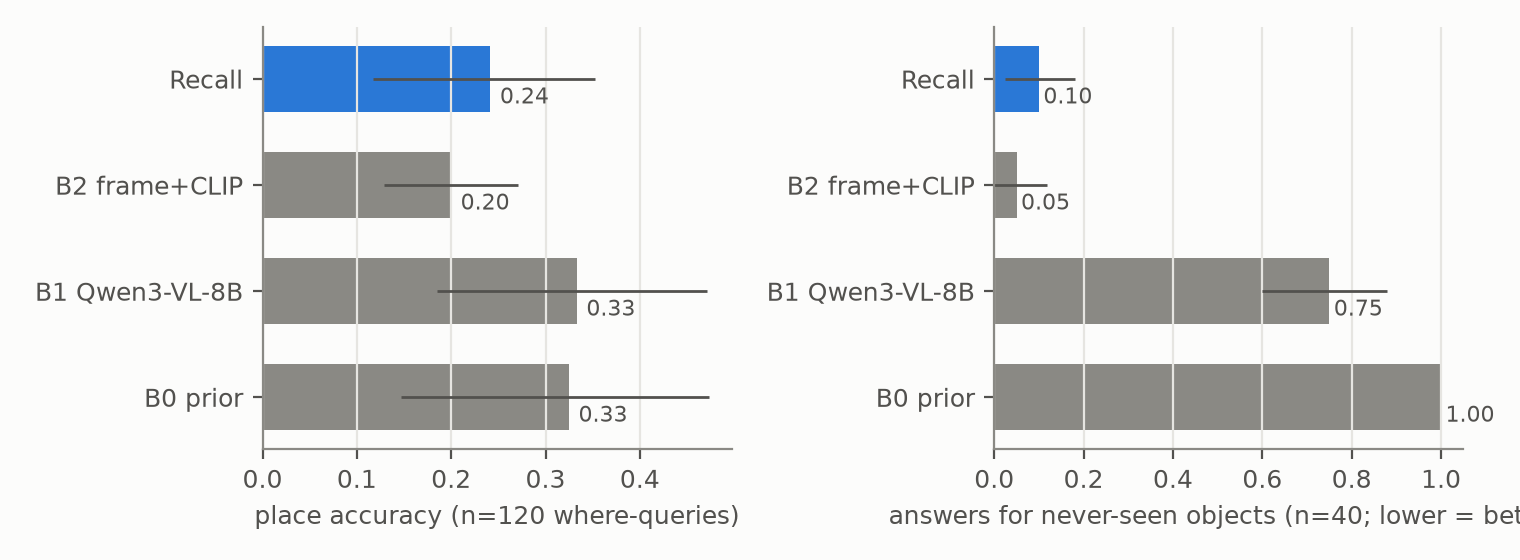
\includegraphics[width=\linewidth]{figs/b1_subsample.png}
\caption{Matched subsample answered by the VLM baseline: accuracy (left), answers for never-seen objects (right).}\label{fig:b1}\end{figure}
Figure~\ref{fig:m1} shows that no perception-based system clears the location prior. On the VLM's subsample
(Fig.~\ref{fig:b1}), Recall's place accuracy is \RecallLocSub{} vs.\ \BoneLoc{} for the VLM (difference
\RecallMinusBone{} [\RecallMinusBoneLo, \RecallMinusBoneHi]); for never-seen objects the VLM names a place
\BoneHall{} of the time and Recall \RecallHallSub{} (difference \HallDiff{} [\HallDiffLo, \HallDiffHi]). Object identity
is the bottleneck: the object head reaches \ObjHeadVal{} top-1 on val over 300 nouns.

% generated — do not edit
\section{Learned Trigger}\label{sec:trigger}\textcolor{red}{[pending]}

\section{Compact Event Memory}\label{sec:memory}\textcolor{red}{[pending]}

\section{Calibrated Answers and Abstention}\label{sec:calib}\textcolor{red}{[pending]}

\section{Compression and On-Device Port}\label{sec:compress}
\begin{figure}[t]\centering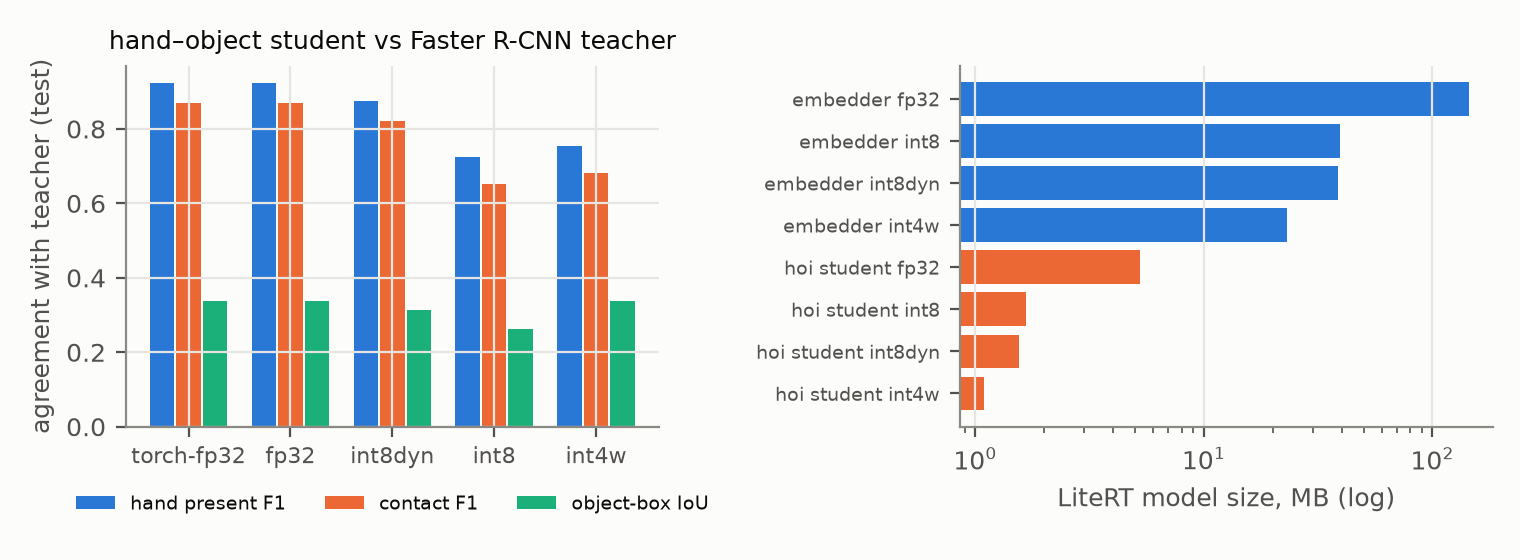
\includegraphics[width=\linewidth]{figs/compression.png}
\caption{Hand--object student agreement with the teacher per precision (left) and LiteRT sizes (right).}\end{figure}
The hand--object student agrees with the Faster R-CNN teacher on held-out frames with hand-present F1 \HoiHandF{} and
contact F1 \HoiContactF{} (\HoiContactFQ{} after dynamic INT8). The embedder goes from \EmbMBfp\,MB to \EmbMBq\,MB with
INT8 weight-only quantisation (cosine to fp32 \EmbCosQ); channel-wise INT4 weights destroy it (cosine \EmbCosFour).
All latency numbers are \emph{desktop-proxy}: no phone was available.

\section{Privacy Layer}\label{sec:privacy}
\begin{figure}[t]\centering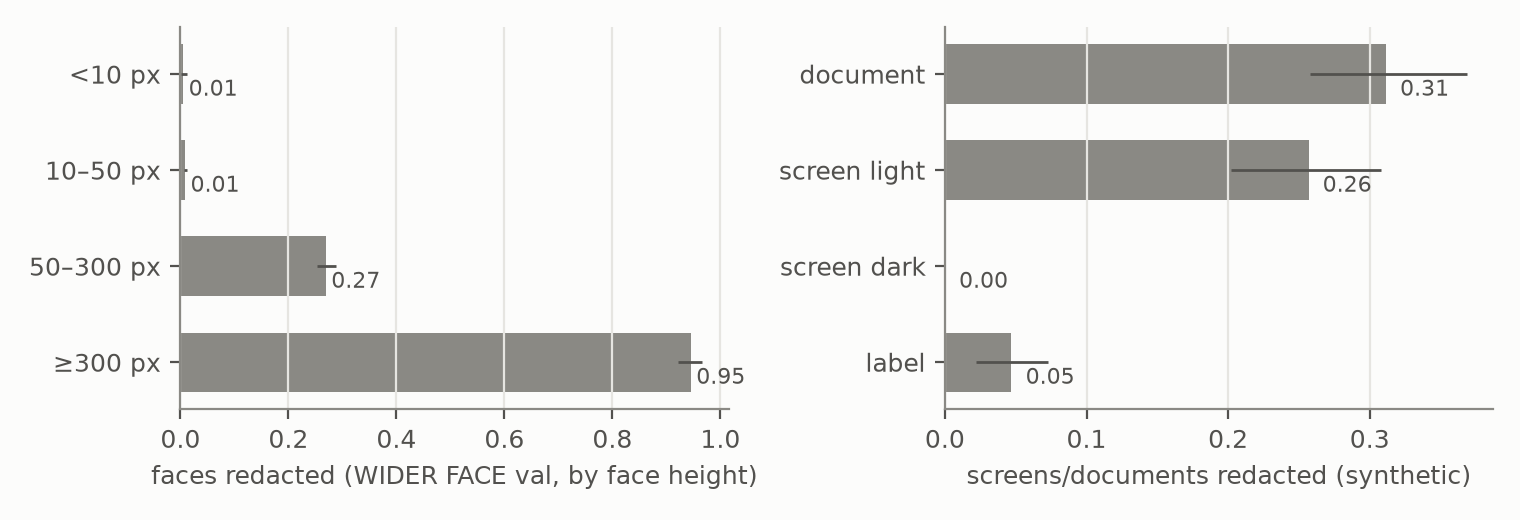
\includegraphics[width=\linewidth]{figs/redaction.png}
\caption{Redaction recall: faces by size (WIDER FACE val) and synthetic screens/documents.}\end{figure}
The redactor catches \FaceLarge{} of faces taller than 300\,px but only \FaceAll{} of all WIDER FACE faces, and
\ScreenAll{} of synthetic screens/documents (none in dark mode). Thumbnails are small event crops, which limits
exposure, but this is the weakest component and is reported as such.

\section{Energy (Estimated)}\label{sec:energy}\textcolor{red}{[pending]}


\section{Limitations and Ethics}
Kitchen narrations cover only narrated interactions and a single room type; there are no official Ego4D numbers, no
real personal recordings and no user-study data yet (the protocol, consent material and analysis are prepared and
validated on simulated participants only). B1 is an open VLM run locally, not a frontier cloud model. Energy is
estimated, not measured. One answer-rule option (place marginalisation over candidate events) was added after a first
test run, re-selected on val for every system, and is disclosed. Redaction misses most small faces and all dark-mode
screens on our proxies; embeddings are computed before redaction. Wearable memory affects bystanders: we never commit
footage, faces or credentials, cloud baselines run only on public data behind an explicit flag, and any deployment needs
consent and visible recording indicators.

{\small\bibliographystyle{plainnat}\bibliography{refs}}
\end{document}
